\documentclass[11pt,a4paper]{article}
%\documentclass[11pt,a4paper,twoside]{article}
\usepackage[utf8]{inputenc}
\usepackage[french]{babel}
\usepackage[T1]{fontenc}

\usepackage{amsmath}
\usepackage{amsfonts}
\usepackage{amssymb}

\newcommand{\TitreMatiere}{Architecture des Ordinateurs}
\newcommand{\TitreSeance}{Conversions des Flottants}
\newcommand{\NumeroTD}{IEEE 754}
\newcommand{\DateCours}{Novembre 2022}
\newcommand{\AnneeScolaire}{2022-2023}
\newcommand{\Organisation}{EPITA}
\newcommand{\NomAuteurA}{Fabrice BOISSIER}
\newcommand{\MailAuteurA}{fabrice.boissier@epita.fr}
\newcommand{\NomAuteurB}{ }
\newcommand{\MailAuteurB}{ }
\newcommand{\DocKeywords}{Architecture}
\newcommand{\DocLangue}{fr} % "en", "fr", ...

\usepackage{MetalCourseBooklet}

% Babel ne traduit pas toujours bien les tableaux et autres
\renewcommand*\frenchfigurename{%
    {\scshape Figure}%
}
\renewcommand*\frenchtablename{%
    {\scshape Tableau}%
}

% Ne pas afficher le numéro de la légende sur tableaux et figures
\captionsetup{format=sanslabel}


\usepackage{xlop}  % Ajout des jolies divisions posées :   \opdiv{25}{7}  \opidiv{25}{7}
%\usepackage{pstricks}  % style pour xlop

\begin{document}

\EncadreTitre

\bigskip


%\begin{center}
%\begin{tabular}{p{5cm} p{11cm}}
%\textbf{Commandes étudiées :} & \texttt{sh}, \texttt{bash}, \texttt{man}, \texttt{ls}, \texttt{mkdir}, \texttt{touch}, \texttt{chmod}, \texttt{mv}, \texttt{rm}, \texttt{rmdir}, \texttt{cat}, \texttt{file}, \texttt{which}, \texttt{which}\\
%
%\textbf{Builtins étudiées :} & \texttt{pwd}, \texttt{cd}, \texttt{exit}, \texttt{logout}, \texttt{echo}, \texttt{umask}, \texttt{type}, \texttt{>}, \texttt{>{}>}, \texttt{<}, \texttt{<{}<}, \texttt{|}\\
%
%\textbf{Notions étudiées :} & Shell, Manuels, Fichiers, Répertoires, Droits, Redirections\\
%\end{tabular}
%\end{center}

\bigskip


Ce document a pour objectif de vous familiariser avec les conversions entre plusieurs bases pour les flottants en respectant la norme IEEE 754.

\bigskip

La plupart des conversions que nous effectuerons seront entre les bases 2, 10, et 16 pour les flottants IEEE 754.

Pour rappel, un nombre en indice peut indiquer la base ($ 10_{2} $ indique du binaire, $ 10_{10} $ indique du décimal, ...) tout comme un symbole en préfixe ($ \% $ indique du binaire, et $ \$ $ indique de l'hexadécimal).
Sans symbole particulier, on considère qu'il s'agit de la base 10 usuelle.

\bigskip

%%%%%%%%%%%%%%%%%%%%%%%%%%%%%%%%%%%%%%

\section{Représentation des flottants}

\bigskip

Les flottants concernent les nombres à virgules.
Représenter et manipuler des nombres à virgules n'est pas aisé dans le sens où plusieurs questions se posent : combien de nombres après la virgule faut-il gérer ? Quel est le plus petit pas/décalage supporté par un ordinateur ? ...
Ces questions touchent au principal problème rencontré par l'informatique dans le traitement des données scientifiques : la \og précision \fg{} .

\bigskip

La précision décrit combien de bits seront utilisés pour représenter les nombres flottants.
Dans la norme IEEE 754, il existe plusieurs formats pour représenter les flottants, dont la \textit{simple précision} (sur 32 bits), la \textit{double précision} (sur 64 bits), et la \textit{double précision étendue} (sur 80 bits).

\bigskip

Parmi les contraintes que vous aviez déjà vus, un nombre entier codé sur 8 bits ne pourra pas aller au delà de la valeur $ 256 $ : si on a $ \% \, 1111 \; 1111 $ et qu'on lui ajoute $ 1 $, alors de la valeur 256, on repassera à 0.
Ce phénomène s'appelle un \textit{integer overflow} (dépassement d'entier), qu'il ne faut pas confondre avec les autres types d'\textit{overflows} (stack overflow, buffer overflow).
Dans le cas des flottants, ce type de dépassement est également possible, mais, il existe également le cas inverse : l'\textit{underflow} où l'on cherche à représenter une valeur trop petite pour la précision choisie.

\medskip

\begin{center}
\begin{figure}[ht!]
\centering{
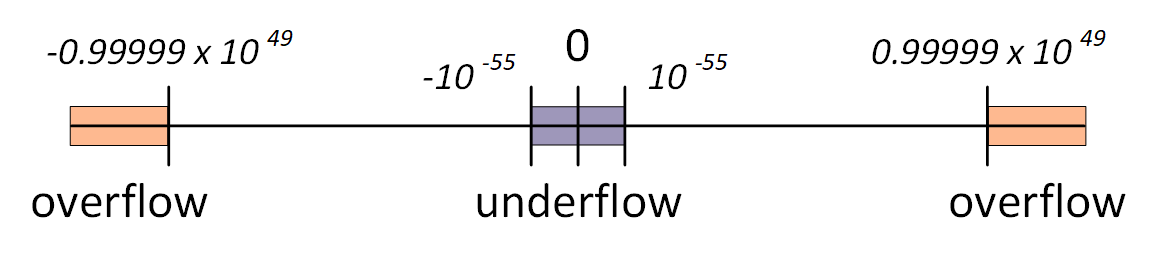
\includegraphics[scale=1]{img/floats_overflows_underflows.png}
\caption{(extrait de \og \textit{Englander: The Architecture of Computer Hardware and Systems Software} \fg{})}
}
\end{figure}
\end{center}

Ainsi, non seulement il existe une limite haute/basse sur la partie entière représentable d'un nombre, mais également sur la quantité de chiffres après la virgule.
Les nombres flottants sont donc parfois des approximations lorsqu'ils sont manipulés.
En développement, on ne teste \textit{jamais} l'égalité entre deux variables représentées par des nombres flottants, mais uniquement un écart entre elles (si cet écart est suffisamment négligeable, alors elles peuvent être considérées comme égales).

\bigskip

Lorsque l'on travaille sur les nombres à virgules, vous connaissez déjà une forme de notation dite scientifique.
On y met un unique entier entre $ 1 $ et $ 9 $ (inclus), et on l'accompagne d'une virgule suivi d'un nombre, puis on le multiplie par une puissance de $ 10 $.

\bigskip

\begin{equation*}
-2541,3945 = -2,5413945 \times 10^{3}
\label{equation:1-Notation-Scientifique}
\end{equation*}

\bigskip

Cette notation est parfois simplifiée en utilisant un $ e $ pour \textit{exposant}.

\bigskip

\begin{equation*}
0,0001337 = 1,337 \times 10^{-4} = 1,337\text{e}-4
\label{equation:2-Notation-Scientifique}
\end{equation*}

\bigskip

Ce format $ \pm \, a \times 10^{n} $ est également utilisé pour représenter les nombres dits flottants (car la virgule \og flotte \fg{} selon la puissance de 10 utilisée).
Cette notation se compose de trois éléments :

\bigskip

%\begin{center}
%\begin{tabular}{c c c c}
%\underline{$\pm$} & \underline{a} & $ \times 10 $ & \underline{$^{n}$} \\
%            signe &      mantisse &               &           exposant \\
%\end{tabular}
%\end{center}

\begin{center}
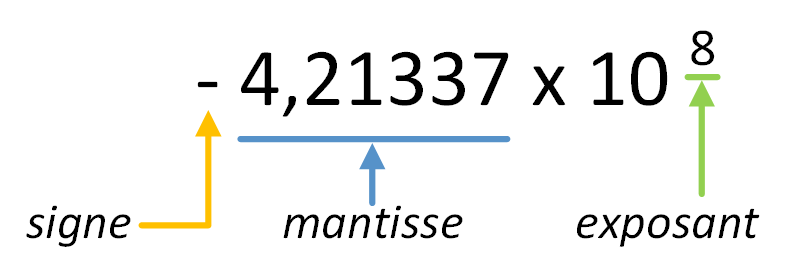
\includegraphics[scale=0.75]{img/floats_parties.png}
\end{center}

\bigskip

\begin{itemize}
\item \textit{signe} : positif ou négatif (ici \og - \fg{})
\item \textit{exposant} : la puissance de 10 (ici $ 8 $)
\item \textit{mantisse} (ou significande) : le nombre décimal (ici $ 4,21337 $)
\end{itemize}

\bigskip

Dans la notation IEEE 754, on utilise ces mêmes concepts, mais appliqués à la base 2 et avec une taille précise pour représenter chacun d'entre eux.
Ainsi, la mantisse a une valeur minimale et une valeur maximale, tout comme l'exposant.
De plus, le vocabulaire varie légèrement du fait que la norme impose quelques contraintes.
On parlera donc dans le vocabulaire formel de :

\bigskip

\begin{itemize}
\item \textit{signe} : positif ou négatif
\item \textit{exposant biaisé} : la puissance de 2, à laquelle il faut ajouter une valeur (le biais)
\item \textit{mantisse} : la partie décimale après la virgule (en ignorant le 1 de la partie entière)
\end{itemize}

\begin{figure}[ht!]
\centering{
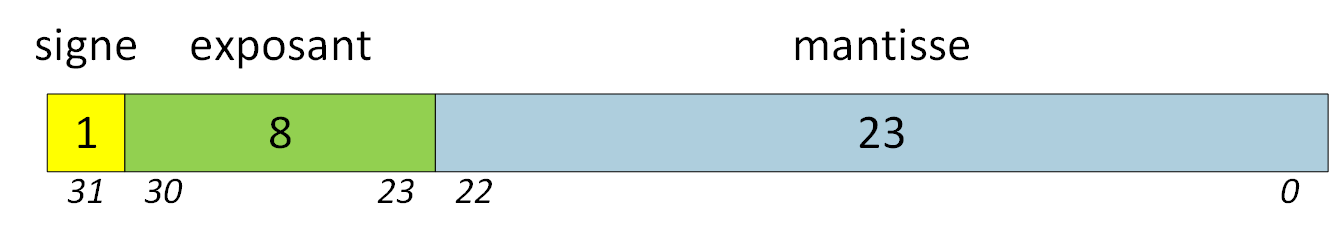
\includegraphics[scale=0.65]{img/floats_precision_single_length.png}
}
\caption{représentation des flottants IEEE 754 simple précision (32 bits)}
\end{figure}

\begin{figure}[ht!]
\centering{
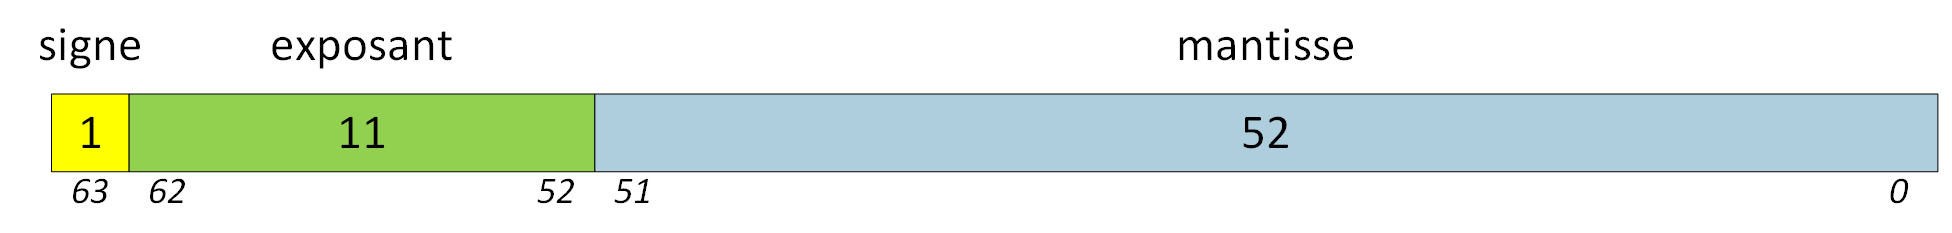
\includegraphics[scale=0.65]{img/floats_precision_double_length.png}
}
\caption{représentation des flottants IEEE 754 double précision (64 bits)}
\end{figure}


\bigskip

De plus, étant donné que les représentations numériques ont des limites, on distingue plusieurs cas dans la taille des flottants : la \textit{simple précision} (ou \textit{single precision} en anglais) sur 32 bits, la \textit{double précision} sur 64 bits, et d'autres formats que nous n'étudierons pas.
La précision fait varier la taille générale des flottants, ce qui implique que les flottants double précision couvreront plus de grandes valeurs, mais également plus de petites valeurs proches de $ 0 $, que les flottants simple précision.

\bigskip

\begin{itemize}
\item \textit{signe} : 1 bit
\item \textit{exposant} : 8 bits (simple précision), 11 bits (double précision), 15 bits (quadruple precision)
\item \textit{mantisse} : 23 bits (simple précision), 52 bits (double précision), 112 bits (quadruple precision)
\end{itemize}

\bigskip

Enfin, pour convertir les décimaux en flottants IEEE 754, il existe une convention pour les \textit{nombres normalisés} (valeur absolue supérieure à 1), et les \textit{nombre dénormalisés} (valeur absolue inférieure à 1).

\bigskip

%%%%%%%%%%%%%%%%%%%%%%%%%%%%%%%%%%%%%%

\section{Valeurs réservées}

\bigskip

La norme prévoit également une réservation de certaines valeurs clés.
Vous devez les connaître pour pouvoir les reconnaître.

\begin{center}
\begin{tabular}{ | c | c | c | c | c | }
\hline
Type & Valeur héxadécimale & Signe & Exposant & Mantisse \\
\hline
+ Zéro      & $ \$ $ 0000 0000 & 0 & $ \% 0000 \, 0000 $ & $ \% \; 000 \, 0000 \, 0000 \, 0000 \, 0000 \, 0000 $ \\
- Zéro      & $ \$ $ 8000 0000 & 1 & $ \% 0000 \, 0000 $ & $ \% \; 000 \, 0000 \, 0000 \, 0000 \, 0000 \, 0000 $ \\
\hline
+ $ \infty $  & $ \$ $ 7F80 0000 & 0 & $ \% 1111 \, 1111 $ & $ \% \; 000 \, 0000 \, 0000 \, 0000 \, 0000 \, 0000 $ \\
- $ \infty $  & $ \$ $ FF80 0000 & 1 & $ \% 1111 \, 1111 $ & $ \% \; 000 \, 0000 \, 0000 \, 0000 \, 0000 \, 0000 $ \\
\hline
NaN (borne B) & $ \$ $ \_F81 0000 & X & $ \% 1111 \, 1111 $ & $ \% \; 000 \, 0000 \, 0000 \, 0000 \, 0000 \, 0001 $ \\
NaN (borne H) & $ \$ $ \_FFF 0000 & X & $ \% 1111 \, 1111 $ & $ \% \; 111 \, 1111 \, 1111 \, 1111 \, 1111 \, 1111 $ \\
\hline
\end{tabular}
\end{center}

\bigskip


%%%%%%%%%%%%%%%%%%%%%%%%%%%%%%%%%%%%%%%%%%%%%%%%%%%%%%%%%%%%%%%%%%%%%%%%%
%%%%%%%%%%%%%%%%%%%%%%%%%%%%%%%%%%%%%%%%%%%%%%%%%%%%%%%%%%%%%%%%%%%%%%%%%
%%%%%%%%%%%%%%%%%%%%%%%%%%%%%%%%%%%%%%%%%%%%%%%%%%%%%%%%%%%%%%%%%%%%%%%%%
%%%%%%%%%%%%%%%%%%%%%%%%%%%%%%%%%%%%%%%%%%%%%%%%%%%%%%%%%%%%%%%%%%%%%%%%%


\section{Nombres normalisés}

\bigskip

Les nombres normalisés dans le format IEEE 754 concernent les nombres dont la valeur absolue est supérieure à $ 1 $ (mais restent inférieurs à la borne maximale gérée par la précision choisie).
L'objectif est de représenter les nombres 
Voici les étapes pour convertir les nombres normalisés :

\medskip

\begin{enumerate}
\item Récupérer le signe du nombre (positif = 0, négatif = 1)
\item Séparer la partie entière de la partie décimale
\item Convertir la partie entière en binaire (sans gérer le signe)
\item Convertir la partie décimale en binaire (sans gérer le signe)
\item Fusion des parties entière et décimale en binaire tout en gardant la virgule
\item Réécriture en notation scientifique base 2
\item Calculer l'exposant pour le format IEEE 754 en l'ajoutant au biais de la précision choisie
\item Convertir l'exposant biaisé en binaire
\item Reporter la mantisse selon la précision choisie
\end{enumerate}

\bigskip

Nous traiterons ici comme exemple la valeur $ - 42,1337 $.

\bigskip

\subsection{Récupérer le signe du nombre}

\medskip

On place dans le bit de poids fort servant à coder le signe un $ 0 $ si le nombre est positif, ou un $ 1 $ si le nombre est négatif.
Dans l'ensemble des étapes suivantes, on peut ignorer le signe du nombre.

\medskip

On retient donc $ 1 $ que l'on place au bit 31 en simple précision, et au bit 63 en double précision.

Pour les étapes suivantes, on travaillera donc sur $ 42,15625 $.

\bigskip

\subsection{Séparer la partie entière de la partie décimale}

\medskip

On sépare la partie entière de la partie décimale afin de les convertir en binaire chacune de leur façon.

\medskip

$ 42,15625 $ devient donc $ 42 $ et $ 0,15625 $.

\bigskip

\subsection{Convertir la partie entière en binaire}

\medskip

On convertit la partie entière en binaire avec l'algorithme classique de division par 2.

\medskip

Dans les traitements suivants, le $ 1 $ de tête sera considéré comme implicite, donc il sera omis lors de l'écriture finale de la mantisse.
Pour le traitement suivant concernant la conversion binaire de la partie décimale, il est parfois utile de connaître le nombre de bits utilisés pour représenter cette partie (moins le $ 1 $ de tête).
Néanmoins, pour connaître le nombre de décalages nécessaires, il est nécessaire de conserver le nombre binaire tel quel.

\medskip

$ 42_{10} \; = \; 101010_{2} $

\bigskip

\subsection{Convertir la partie décimale en binaire}

\medskip

On convertit la partie décimale en binaire.
Pour cela, on effectue des multiplications successives par $ 2 $ en faisant l'extraction de la partie entière.
En effet, les bits représentent toujours des puissances de 2, mais des puissances négatives (donc $ 2^{-1} $, $ 2^{-2} $, $ 2^{-3} $, ... soit $ 0,5 $, $ 0,25 $, $ 0,125 $, ...).

\medskip

La condition d'arrêt est soit d'atteindre $ 1,0 $, soit que la taille de la partie entière convertie en binaire + le nombre de multiplication tienne sur la taille de la mantisse exploitée.
Dans notre cas, $ 42 $ est converti en $ 101010_{2} $, donc en omettant le $ 1 $ de tête, $ 01010_{2} $, celui-ci prendra 5 bits dans la mantisse.
En simple précision, la mantisse étant de 23 bits, on pourra donc placer 18 bits ($ 23 - 5 $) de nombres après la virgule.
À la fin de la dernière multiplication applicable (la $ 18^e $), on arrondit le résultat à $ 0 $ ou $ 1 $.

\medskip

\begin{center}
\begin{tabular}{c c c   m{1cm}   c }
multiplication        &         & résultat    & & entier \\
$ 0,15625 \times 2 $  &  $ = $  &  $ 0,31250 $ & & $ 0 $ \\
$ 0,3125  \times 2 $  &  $ = $  &  $ 0,6250  $ & & $ 0 $ \\
$ 0,625   \times 2 $  &  $ = $  &  $ 1,250   $ & & $ 1 $ \\
$ 0,25    \times 2 $  &  $ = $  &  $ 0,50    $ & & $ 0 $ \\
$ 0,5     \times 2 $  &  $ = $  &  $ 1,0     $ & & $ 1 $ \\
\end{tabular}
\end{center}

\medskip

On lit cette fois les multiplications dans l'ordre où elles ont été effectuées.

\medskip

$ 0,15625_{10} = 0,00101_{2} $

%\begin{tabular}{c c c   m{1cm}   c }
%multiplication       &         & résultat    & & entier
%$ 0,1337 \times 2 $  &  $ = $  &  $ 0,2674 $ & & $ 0 $
%$ 0,2674 \times 2 $  &  $ = $  &  $ 0,5348 $ & & $ 0 $
%$ 0,5348 \times 2 $  &  $ = $  &  $ 1,0696 $ & & $ 1 $
%$ 0,0696 \times 2 $  &  $ = $  &  $ 0,1392 $ & & $ 0 $
%$ 0,1392 \times 2 $  &  $ = $  &  $ 0,2784 $ & & $ 0 $
%$ 0,2784 \times 2 $  &  $ = $  &  $ 0,5568 $ & & $ 0 $
%$ 0,5568 \times 2 $  &  $ = $  &  $ 1,1136 $ & & $ 1 $
%$ 0,1136 \times 2 $  &  $ = $  &  $ 0,2272 $ & & $ 0 $
%$ 0,2272 \times 2 $  &  $ = $  &  $ 0,4544 $ & & $ 0 $
%$ 0,4544 \times 2 $  &  $ = $  &  $ 0,9088 $ & & $ 0 $
%$ 0,9088 \times 2 $  &  $ = $  &  $ 1,8176 $ & & $ 1 $
%$ 0,8176 \times 2 $  &  $ = $  &  $ 1,6352 $ & & $ 1 $
%$ 0,6352 \times 2 $  &  $ = $  &  $ 1,2704 $ & & $ 1 $
%$ 0,2704 \times 2 $  &  $ = $  &  $ 0,5408 $ & & $ 0 $
%$ 0,5408 \times 2 $  &  $ = $  &  $ 1,0816 $ & & $ 1 $
%$ 0,0816 \times 2 $  &  $ = $  &  $ 0,1632 $ & & $ 0 $
%$ 0,1632 \times 2 $  &  $ = $  &  $ 0,3264 $ & & $ 0 $
%$ 0,3264 \times 2 $  &  $ = $  &  $ 0,6528 $ & & $ 0 $ <= 1 arrondi au dessus ?
%$ 0,6528 \times 2 $  &  $ = $  &  $ 1,3056 $ & & $ 1 $
%\end{tabular}

% You entered                     : -42.1337
% Value actually stored in float  : -42.133701324462890625
% Error due to conversion         : -0.000001324462890625
% Binary Representation           : 1 10000100 01010001000100011101001
% Binary Representation           : 1 10000100 01010,001000100011101001
% Binary Representation           : 11000010001010001000100011101001
% Hexadecimal Representation      : 0xc22888e9


\bigskip

\subsection{Fusion des parties entière et décimale en binaire tout en gardant la virgule}

\medskip

On fusionne les parties entières et décimales converties en binaire, tout en conservant le placement de la virgule.

\medskip

$ 42_{10} = 101010_{2} $

\medskip

$ 0,15625_{10} = 0,00101_{2} $

\bigskip

$ 42,15625_{10} = 101010,00101_{2} $

\bigskip

\subsection{Réécriture en notation scientifique base 2}

\medskip

On déplace la virgule pour atteindre le $ 1 $ le plus à gauche de la partie entière, et on garde ce décalage comme exposant.

\medskip

$ 101010,00101_{2} = 1,0101000101 \times 2^{5} $

\bigskip

\subsection{Calculer l'exposant en ajoutant le biais}

\medskip

On ajoute le biais (lié à la précision choisie) à l'exposant précédemment obtenu.
En simple précision, le biais est de $ 127 $. En double précision il est de $ 1023 $. En quadruple précision, il est de $ 16383 $.

\medskip

$ 1,0101000101 \times 2^{5} $

\medskip

Simple précision : $ 5 + 127 = 132 $

\medskip

Double précision : $ 5 + 1023 = 1028 $

\bigskip

\subsection{Convertir l'exposant biaisé en binaire}

\medskip

On convertit en binaire l'exposant, et on le reporte dans le champ prévu.

\medskip

Simple précision (8 bits) : $ 132_{10} = \; 1000 \; 0100_{2} $

\medskip

Double précision (11 bits) : $ 1028_{10} = \; 100 \; 0000 \; 0100_{2} $

\bigskip

\subsection{Reporter la mantisse selon la précision choisie}

\medskip

On reporte la mantisse dans le champ prévu en omettant le $ 1 $ en tête : en effet, celui-ci est implicite par l'écriture scientifique en base 2.

De plus, on ajoute autant de $ 0 $ que nécessaire à droite du nombre.

\medskip

$ 1,0101000101_{2} \times 2^{5} $

\medskip

$ 0101000101_{2} $

\medskip

Simple précision (23 bits) :

$ 0101 0001 0100 0000 0000 000_{2} $

\medskip

Double précision (52 bits) :

$ 0101 0001 0100 0000 0000 0000 0000 0000 0000 0000 0000 0000 0000_{2} $

\bigskip

\subsection{Résultat}

\bigskip

Enfin, on peut fusionner l'ensemble des champs pour représenter un nombre normalisé au format IEEE 754 : signe ($ 1 $), exposant ($ 1000 0100_{2} $ ou $ 100 0000 0100_{2} $), mantisse

\medskip


Simple précision (32 bits) :

$ 1 1000 0100 0101 0001 0100 0000 0000 000_{2} $

\medskip

Double précision (64 bits) :

$ 1 100 0000 0100 0101 0001 0100 0000 0000 0000 0000 0000 0000 0000 0000 0000 0000_{2} $


\bigskip


Simple précision (32 bits) : $ -42.15625_{10} = \text{C}228\text{A}000_{16} $

\medskip

Double précision (64 bits) : $ -42.15625_{10} = \text{C}045140000000000_{16} $


% You entered                     : -42.15625
% Value actually stored in float  : -42.15625
% Error due to conversion         : 0.00000
% Binary Representation           : 1 10000100 01010001010000000000000
% Binary Representation           : 11000010001010001010000000000000
% Hexadecimal Representation      : 0xc228a000

\bigskip

%%%%%%%%%%%%%%%%%%%%%%%%%%%%%%%%%%%%%%%%%%%%%%%%%%%%%%%%%%%%%%%%%%%%%%%%%
%%%%%%%%%%%%%%%%%%%%%%%%%%%%%%%%%%%%%%%%%%%%%%%%%%%%%%%%%%%%%%%%%%%%%%%%%
%%%%%%%%%%%%%%%%%%%%%%%%%%%%%%%%%%%%%%%%%%%%%%%%%%%%%%%%%%%%%%%%%%%%%%%%%
%%%%%%%%%%%%%%%%%%%%%%%%%%%%%%%%%%%%%%%%%%%%%%%%%%%%%%%%%%%%%%%%%%%%%%%%%

\section{Nombres dénormalisés}

\bigskip

Les nombres dénormalisés (\textit{subnormal numbers}, \textit{denormalized numbers}, ou \textit{denormals} en anglais) concernent les nombres dont la valeur absolue est strictement inférieure strictement à $ 1 $ (c'est-à-dire les nombres tels que : $ -1 < n < 1 $).
Comme ces nombres ont un $ 0 $ comme chiffre entier, on ne peut pas les représenter avec une mantisse dont un  $ 1 $ est implicite.
%Ainsi, le format de sortie en binaire change.

\medskip

Dans le format binaire, on reconnait un nombre comme dénormalisé si son exposant est nul (il ne contient que des $ 0 $).

\medskip

Nous ne verrons pas en détails comment obtenir ces nombres, mais vous devrez savoir les repérer.

%Étapes pour les nombres dénormalisés (très proches de 0) : ATTENTION, L'EXPOSANT EST TOUJOURS A 0

%\begin{enumerate}
%\item ???
%\end{enumerate}

\bigskip

\begin{center}
\textit{Ce document et ses illustrations ont été réalisés par Fabrice BOISSIER en novembre 2022}
\end{center}

\end{document}
